\documentclass[tikz,border=2pt,11pt]{standalone}
\usetikzlibrary{positioning}
\usetikzlibrary{arrows.meta}
\usetikzlibrary{calc}
\usetikzlibrary{fit}
\usetikzlibrary{decorations.pathreplacing}
\usepackage{amsmath}
\usepackage{amssymb}
\usepackage{xcolor}
\usepackage{tikz}
\DeclareMathOperator{\diam}{diam}
\DeclareMathOperator{\id}{id}
\DeclareMathOperator{\sht}{ht}
\begin{document}
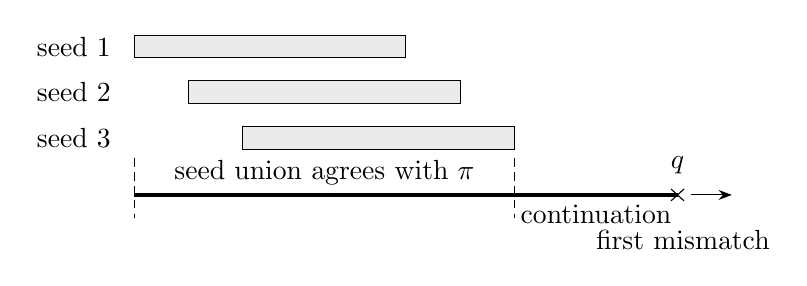
\begin{tikzpicture}[x=0.69cm,y=0.58cm,>=Stealth]
  \draw[fill=black!8] (1,2) rectangle (6,2.5);
  \draw[fill=black!8] (2,1) rectangle (7,1.5);
  \draw[fill=black!8] (3,0) rectangle (8,0.5);
  \node[anchor=east] at (0.75,2.25) {seed 1};
  \node[anchor=east] at (0.75,1.25) {seed 2};
  \node[anchor=east] at (0.75,0.25) {seed 3};
  \draw[densely dashed] (1,-0.2) -- (1,-1.5);
  \draw[densely dashed] (8,-0.2) -- (8,-1.5);
  \draw[very thick] (1,-1) -- (11,-1);
  \draw[->] (11.25,-1) -- (12,-1);
  \node[above] at (4.5,-1) {seed union agrees with $\pi$};
  \node[below] at (9.5,-1) {continuation};
  \draw (10.88,-1.13) -- (11.12,-0.87);
  \draw (10.88,-0.87) -- (11.12,-1.13);
  \node[above] at (11,-0.75) {$q$};
  \node[below] at (11.1,-1.55) {first mismatch};
\end{tikzpicture}
\end{document}
